\documentclass[14pt]{extbook}
\usepackage{multicol, enumerate, enumitem, hyperref, color, soul, setspace, parskip, fancyhdr} %General Packages
\usepackage{amssymb, amsthm, amsmath, latexsym, units, mathtools} %Math Packages
\everymath{\displaystyle} %All math in Display Style
% Packages with additional options
\usepackage[headsep=0.5cm,headheight=12pt, left=1 in,right= 1 in,top= 1 in,bottom= 1 in]{geometry}
\usepackage[usenames,dvipsnames]{xcolor}
\usepackage{dashrule}  % Package to use the command below to create lines between items
\newcommand{\litem}[1]{\item#1\hspace*{-1cm}\rule{\textwidth}{0.4pt}}
\pagestyle{fancy}
\lhead{Progress Quiz 7}
\chead{}
\rhead{Version A}
\lfoot{4173-5738}
\cfoot{}
\rfoot{Spring 2021}
\begin{document}

\begin{enumerate}
\litem{
First, find the equation of the line containing the two points below. Then, write the equation as $ y=mx+b $ and choose the intervals that contain $m$ and $b$.\[ (7, 2) \text{ and } (-10, -7) \]\begin{enumerate}[label=\Alph*.]
\item \( m \in [-0.14, 1.31] \hspace*{3mm} b \in [0.34, 2.26] \)
\item \( m \in [-1.13, -0.17] \hspace*{3mm} b \in [-13.05, -12.17] \)
\item \( m \in [-0.14, 1.31] \hspace*{3mm} b \in [-2.43, -1.07] \)
\item \( m \in [-0.14, 1.31] \hspace*{3mm} b \in [2.86, 3.56] \)
\item \( m \in [-0.14, 1.31] \hspace*{3mm} b \in [-5.17, -4.93] \)

\end{enumerate} }
\litem{
Write the equation of the line in the graph below in Standard form $Ax+By=C$. Then, choose the intervals that contain $A, B, \text{ and } C$.
\begin{center}
    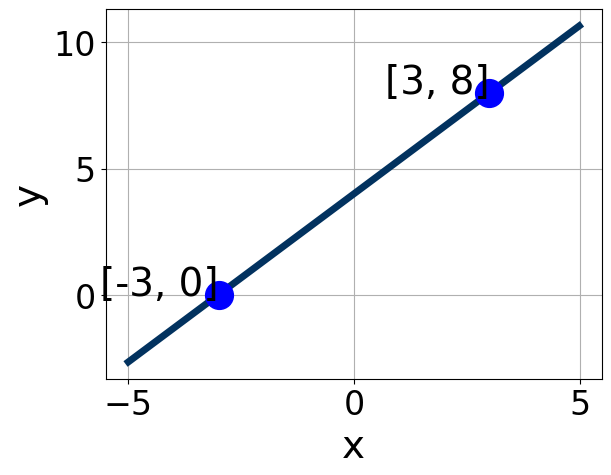
\includegraphics[width=0.5\textwidth]{../Figures/linearGraphToStandardA.png}
\end{center}
\begin{enumerate}[label=\Alph*.]
\item \( A \in [-3.33, 1.67], \hspace{3mm} B \in [-1.66, -0.74], \text{ and } \hspace{3mm} C \in [-7, -1] \)
\item \( A \in [2, 6], \hspace{3mm} B \in [1.52, 4.96], \text{ and } \hspace{3mm} C \in [11, 14] \)
\item \( A \in [-4, -2], \hspace{3mm} B \in [1.52, 4.96], \text{ and } \hspace{3mm} C \in [11, 14] \)
\item \( A \in [2, 6], \hspace{3mm} B \in [-4.58, -1.64], \text{ and } \hspace{3mm} C \in [-15, -10] \)
\item \( A \in [-3.33, 1.67], \hspace{3mm} B \in [-0.08, 1.53], \text{ and } \hspace{3mm} C \in [2, 9] \)

\end{enumerate} }
\litem{
Solve the equation below. Then, choose the interval that contains the solution.\[ -7(-2x -3) = -19(-11x + 17) \]\begin{enumerate}[label=\Alph*.]
\item \( x \in [1.42, 1.74] \)
\item \( x \in [1.23, 1.49] \)
\item \( x \in [-1.72, -1.48] \)
\item \( x \in [1.67, 1.78] \)
\item \( \text{There are no real solutions.} \)

\end{enumerate} }
\litem{
Solve the equation below. Then, choose the interval that contains the solution.\[ -7(9x -14) = -19(2x -4) \]\begin{enumerate}[label=\Alph*.]
\item \( x \in [6.7, 8.3] \)
\item \( x \in [-7.9, -6.2] \)
\item \( x \in [-0.7, 1.4] \)
\item \( x \in [1.5, 2] \)
\item \( \text{There are no real solutions.} \)

\end{enumerate} }
\litem{
Find the equation of the line described below. Write the linear equation as $ y=mx+b $ and choose the intervals that contain $m$ and $b$.\[ \text{Parallel to } 3 x + 4 y = 6 \text{ and passing through the point } (7, 2). \]\begin{enumerate}[label=\Alph*.]
\item \( m \in [-1.18, -0.1] \hspace*{3mm} b \in [-5.6, -3.9] \)
\item \( m \in [-1.18, -0.1] \hspace*{3mm} b \in [-9, -7.2] \)
\item \( m \in [0.38, 1.13] \hspace*{3mm} b \in [-3.3, -0.4] \)
\item \( m \in [-1.82, -0.97] \hspace*{3mm} b \in [5.2, 8.2] \)
\item \( m \in [-1.18, -0.1] \hspace*{3mm} b \in [5.2, 8.2] \)

\end{enumerate} }
\litem{
First, find the equation of the line containing the two points below. Then, write the equation as $ y=mx+b $ and choose the intervals that contain $m$ and $b$.\[ (2, 3) \text{ and } (-7, -4) \]\begin{enumerate}[label=\Alph*.]
\item \( m \in [0.6, 2.4] \hspace*{3mm} b \in [0.88, 1.18] \)
\item \( m \in [0.6, 2.4] \hspace*{3mm} b \in [-1.87, -1.28] \)
\item \( m \in [0.6, 2.4] \hspace*{3mm} b \in [2.89, 3.3] \)
\item \( m \in [-2.6, -0.5] \hspace*{3mm} b \in [-9.47, -9.35] \)
\item \( m \in [0.6, 2.4] \hspace*{3mm} b \in [1.32, 1.63] \)

\end{enumerate} }
\litem{
Find the equation of the line described below. Write the linear equation as $ y=mx+b $ and choose the intervals that contain $m$ and $b$.\[ \text{Perpendicular to } 5 x + 6 y = 15 \text{ and passing through the point } (-2, -6). \]\begin{enumerate}[label=\Alph*.]
\item \( m \in [0.86, 1.29] \hspace*{3mm} b \in [3.31, 3.6] \)
\item \( m \in [-1.6, -1.11] \hspace*{3mm} b \in [-8.41, -8.28] \)
\item \( m \in [0.86, 1.29] \hspace*{3mm} b \in [-4.35, -3.66] \)
\item \( m \in [0.86, 1.29] \hspace*{3mm} b \in [-3.69, -3.22] \)
\item \( m \in [0.67, 0.99] \hspace*{3mm} b \in [-3.69, -3.22] \)

\end{enumerate} }
\litem{
Solve the linear equation below. Then, choose the interval that contains the solution.\[ \frac{-3x -6}{8} - \frac{-5x -8}{4} = \frac{3x + 4}{7} \]\begin{enumerate}[label=\Alph*.]
\item \( x \in [4.2, 5.5] \)
\item \( x \in [-1.3, 1.4] \)
\item \( x \in [-1.8, -1.3] \)
\item \( x \in [7.2, 9.1] \)
\item \( \text{There are no real solutions.} \)

\end{enumerate} }
\litem{
Solve the linear equation below. Then, choose the interval that contains the solution.\[ \frac{-5x + 7}{6} - \frac{5x + 6}{5} = \frac{-5x -5}{2} \]\begin{enumerate}[label=\Alph*.]
\item \( x \in [-3.8, -3.3] \)
\item \( x \in [-7.4, -5.9] \)
\item \( x \in [-11.3, -7.4] \)
\item \( x \in [-0.2, 0.8] \)
\item \( \text{There are no real solutions.} \)

\end{enumerate} }
\litem{
Write the equation of the line in the graph below in Standard form $Ax+By=C$. Then, choose the intervals that contain $A, B, \text{ and } C$.
\begin{center}
    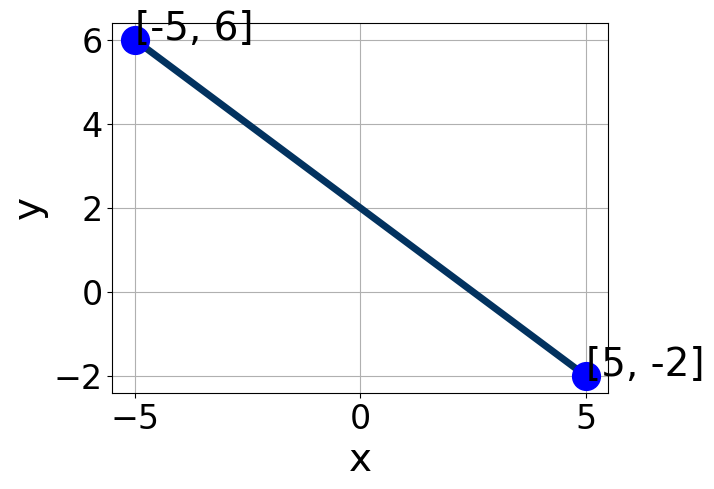
\includegraphics[width=0.5\textwidth]{../Figures/linearGraphToStandardCopyA.png}
\end{center}
\begin{enumerate}[label=\Alph*.]
\item \( A \in [2, 7], \hspace{3mm} B \in [-7.8, -4.9], \text{ and } \hspace{3mm} C \in [-11, -4] \)
\item \( A \in [-1.2, 3.8], \hspace{3mm} B \in [-0.4, 2.9], \text{ and } \hspace{3mm} C \in [2, 8] \)
\item \( A \in [-1.2, 3.8], \hspace{3mm} B \in [-3.9, -0.4], \text{ and } \hspace{3mm} C \in [-2, -1] \)
\item \( A \in [2, 7], \hspace{3mm} B \in [3, 5.7], \text{ and } \hspace{3mm} C \in [7, 11] \)
\item \( A \in [-14, -2], \hspace{3mm} B \in [-7.8, -4.9], \text{ and } \hspace{3mm} C \in [-11, -4] \)

\end{enumerate} }
\end{enumerate}

\end{document}